\section{LHCb Experiment}
%The physics aims of the LHCb experiment are ...

% The LHCb exp. is a SAFS shown in figure X. protons collide on the left then stuff travels through the detector through a series of sub detectors


% The detector was designed around the requirements needed to precisely measure b-hadron decays



% In proton collisions bbbar pais are boosted along the beam pipe so LHCb was deigned only to look at a small angular acceptance

The angular acceptance of the LHCb detector reflects the angular distribution of \bbbar pairs produced in high energy proton collisions. \bbbar pair are produced in this way and are in cones along the beam pipe. Therefore the angualr acceptance of the LHCb detector was chosen to be ... for good study of b hadrons and efficiency use of space and money.
OR
In proton collisions at high energies \bbbar pairs produced are boosted along the beam pipe in either the forwards or backwards direction, the LHCb detector was designed with this in mind. The angular coverage of the detector is from 10 to 250 mrad in the vertical direction and from 10 to 300 mrad in the horizontal direction, the central acceptance is limited by the presence of the beampipe. 


The detector's angular acceptance covers only a small fraction of the 4$\pi$ angular coverage of the general purpose detectors, however approximately 40 $\%$ of $b$-hadron produced are within it's angular accetpance. 

% LHCb operates at a lower luminoscity to reduce pile uip and all for easier analysis of stuff. This is acheived by defocusing the beam.

%Need good vertex and momentum resolution which gives proper time and mass resolutions. Thsi helps the study of occillating Bs system and mass distinguishes btwn signal and background. This is acheive by the sub detectors focuese on tracking ...

% Excellent particle identification is needed to reconstruct the many different final states that b-hadrons can decay into. This is acheived by the ....

% Cannot store all the data so need a good trigger for b=hadrons, relise on some fast infor from parts of the detector. Also event filters?

% The next few sections describe ...


The LHCb experiment was designed to search for indirect evidence of New Physics processes through the study of CP violation and rare decays of hadrons containing $b$ or $c$ quarks. It was built as a single arm forward spectrometer as shown in Figure \ref{fig:LHCb_detector}. The $b$-hadrons are produced on the left of the diagram at the interaction point and the different sub-detectors record signatures of the $b$ hadrons and their decay products as they travel through the detector. The physics aims of the experiment are reflected in various aspects of the detector design. 




\begin{figure}[tb] 
  \centering    
  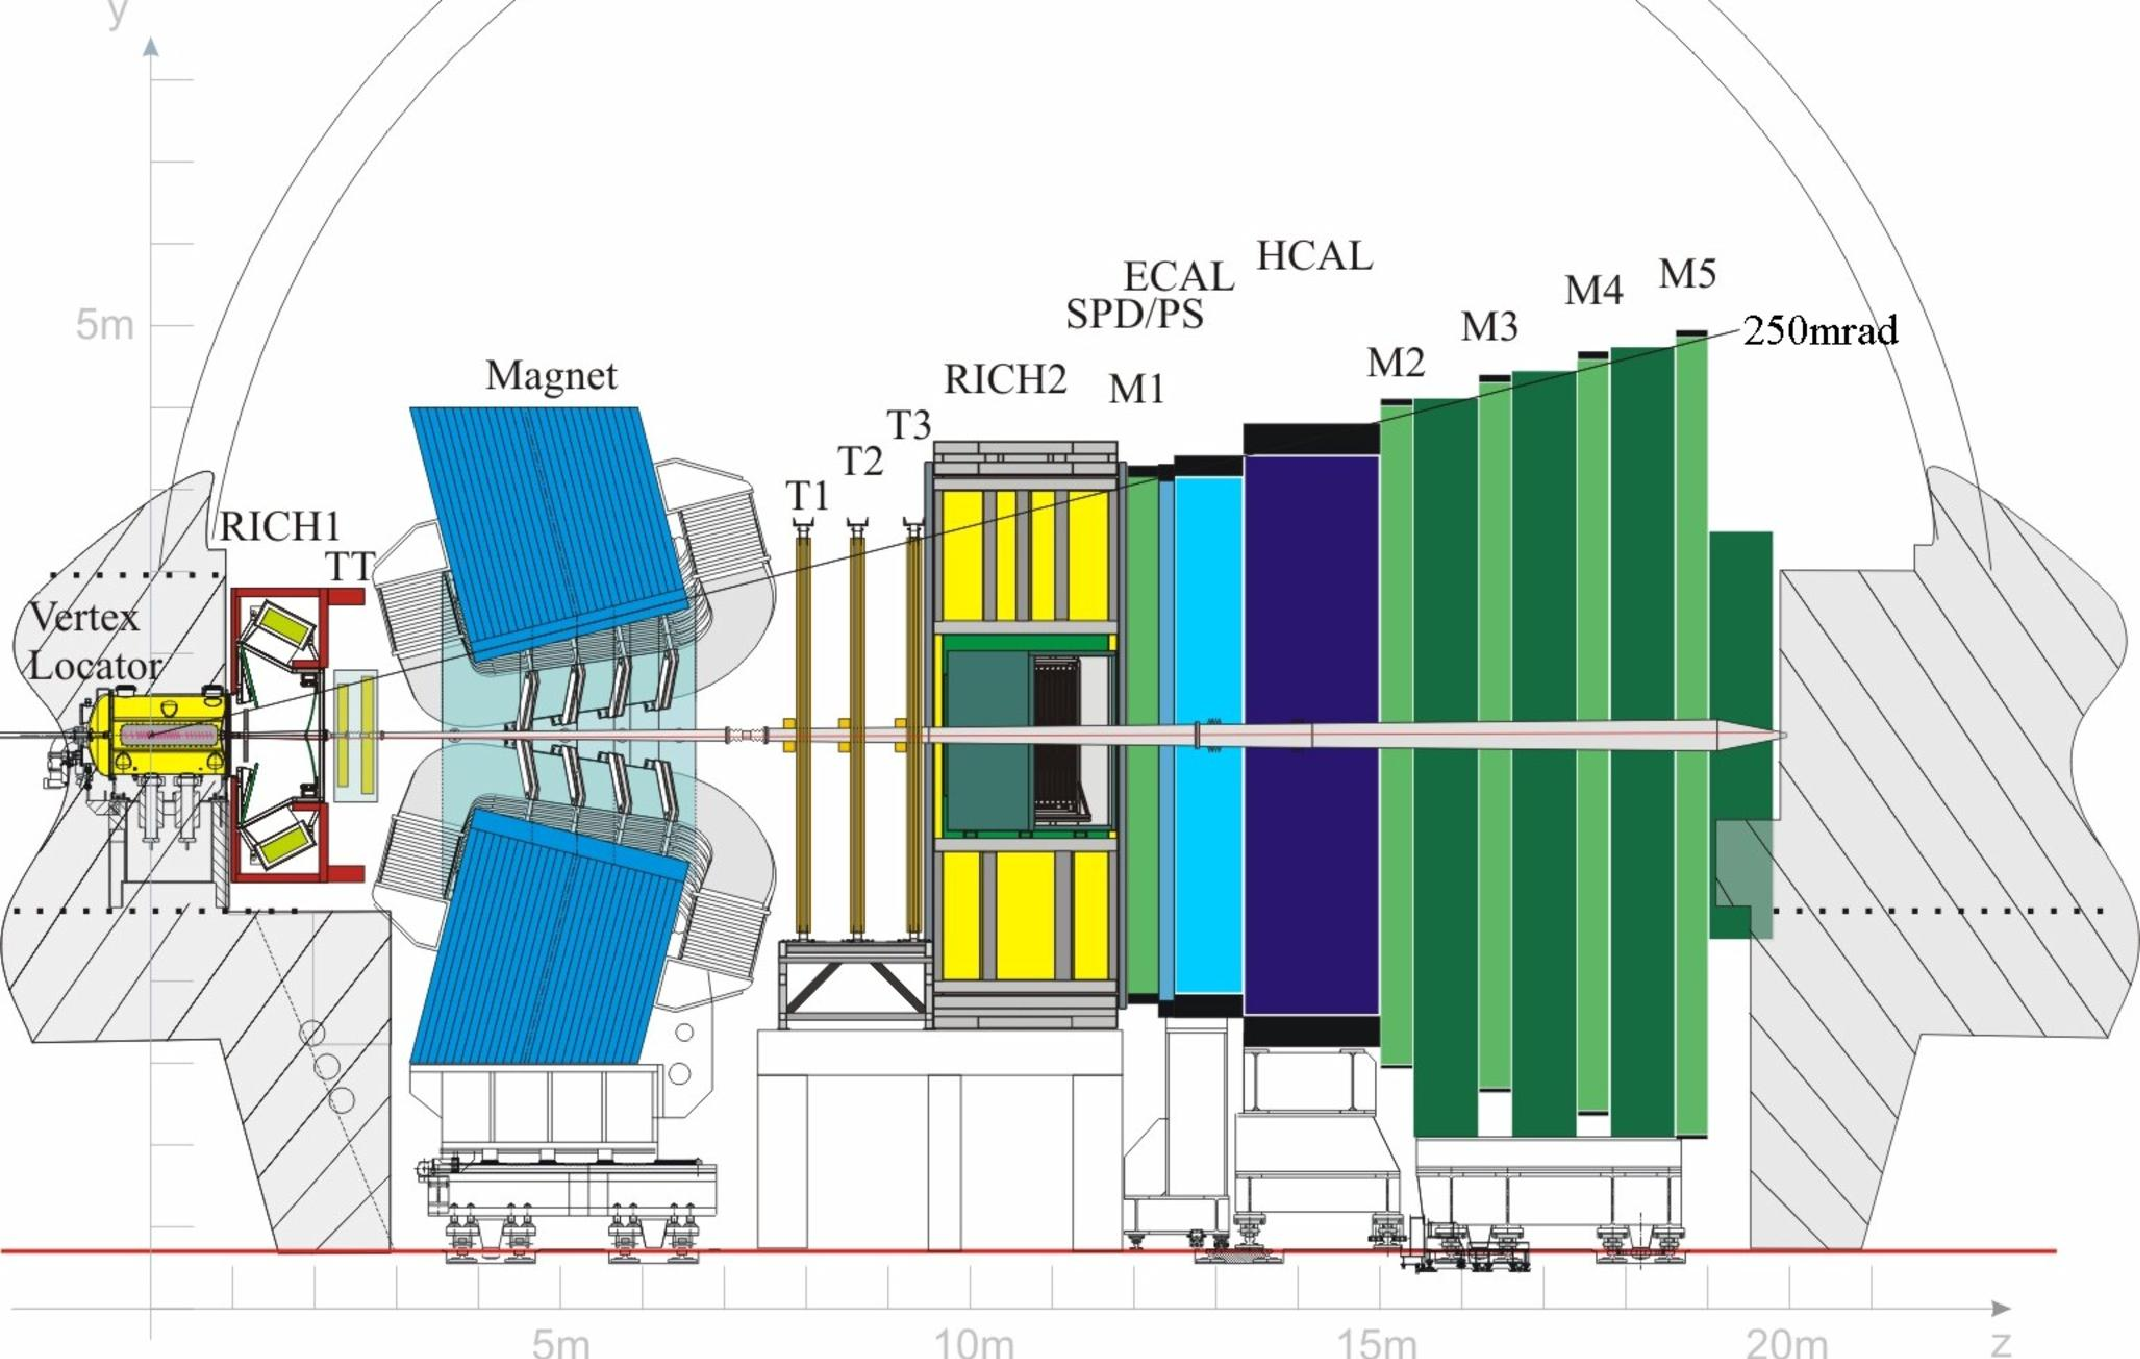
\includegraphics[ width=1.0\textwidth]{LHCb_layout.png}
  \caption{Cross section of the LHCb detector \cite{LHCb:2003ab}.}
  \label{fig:LHCb_detector}
\end{figure}




\begin{figure}[tb] 
  \centering    
  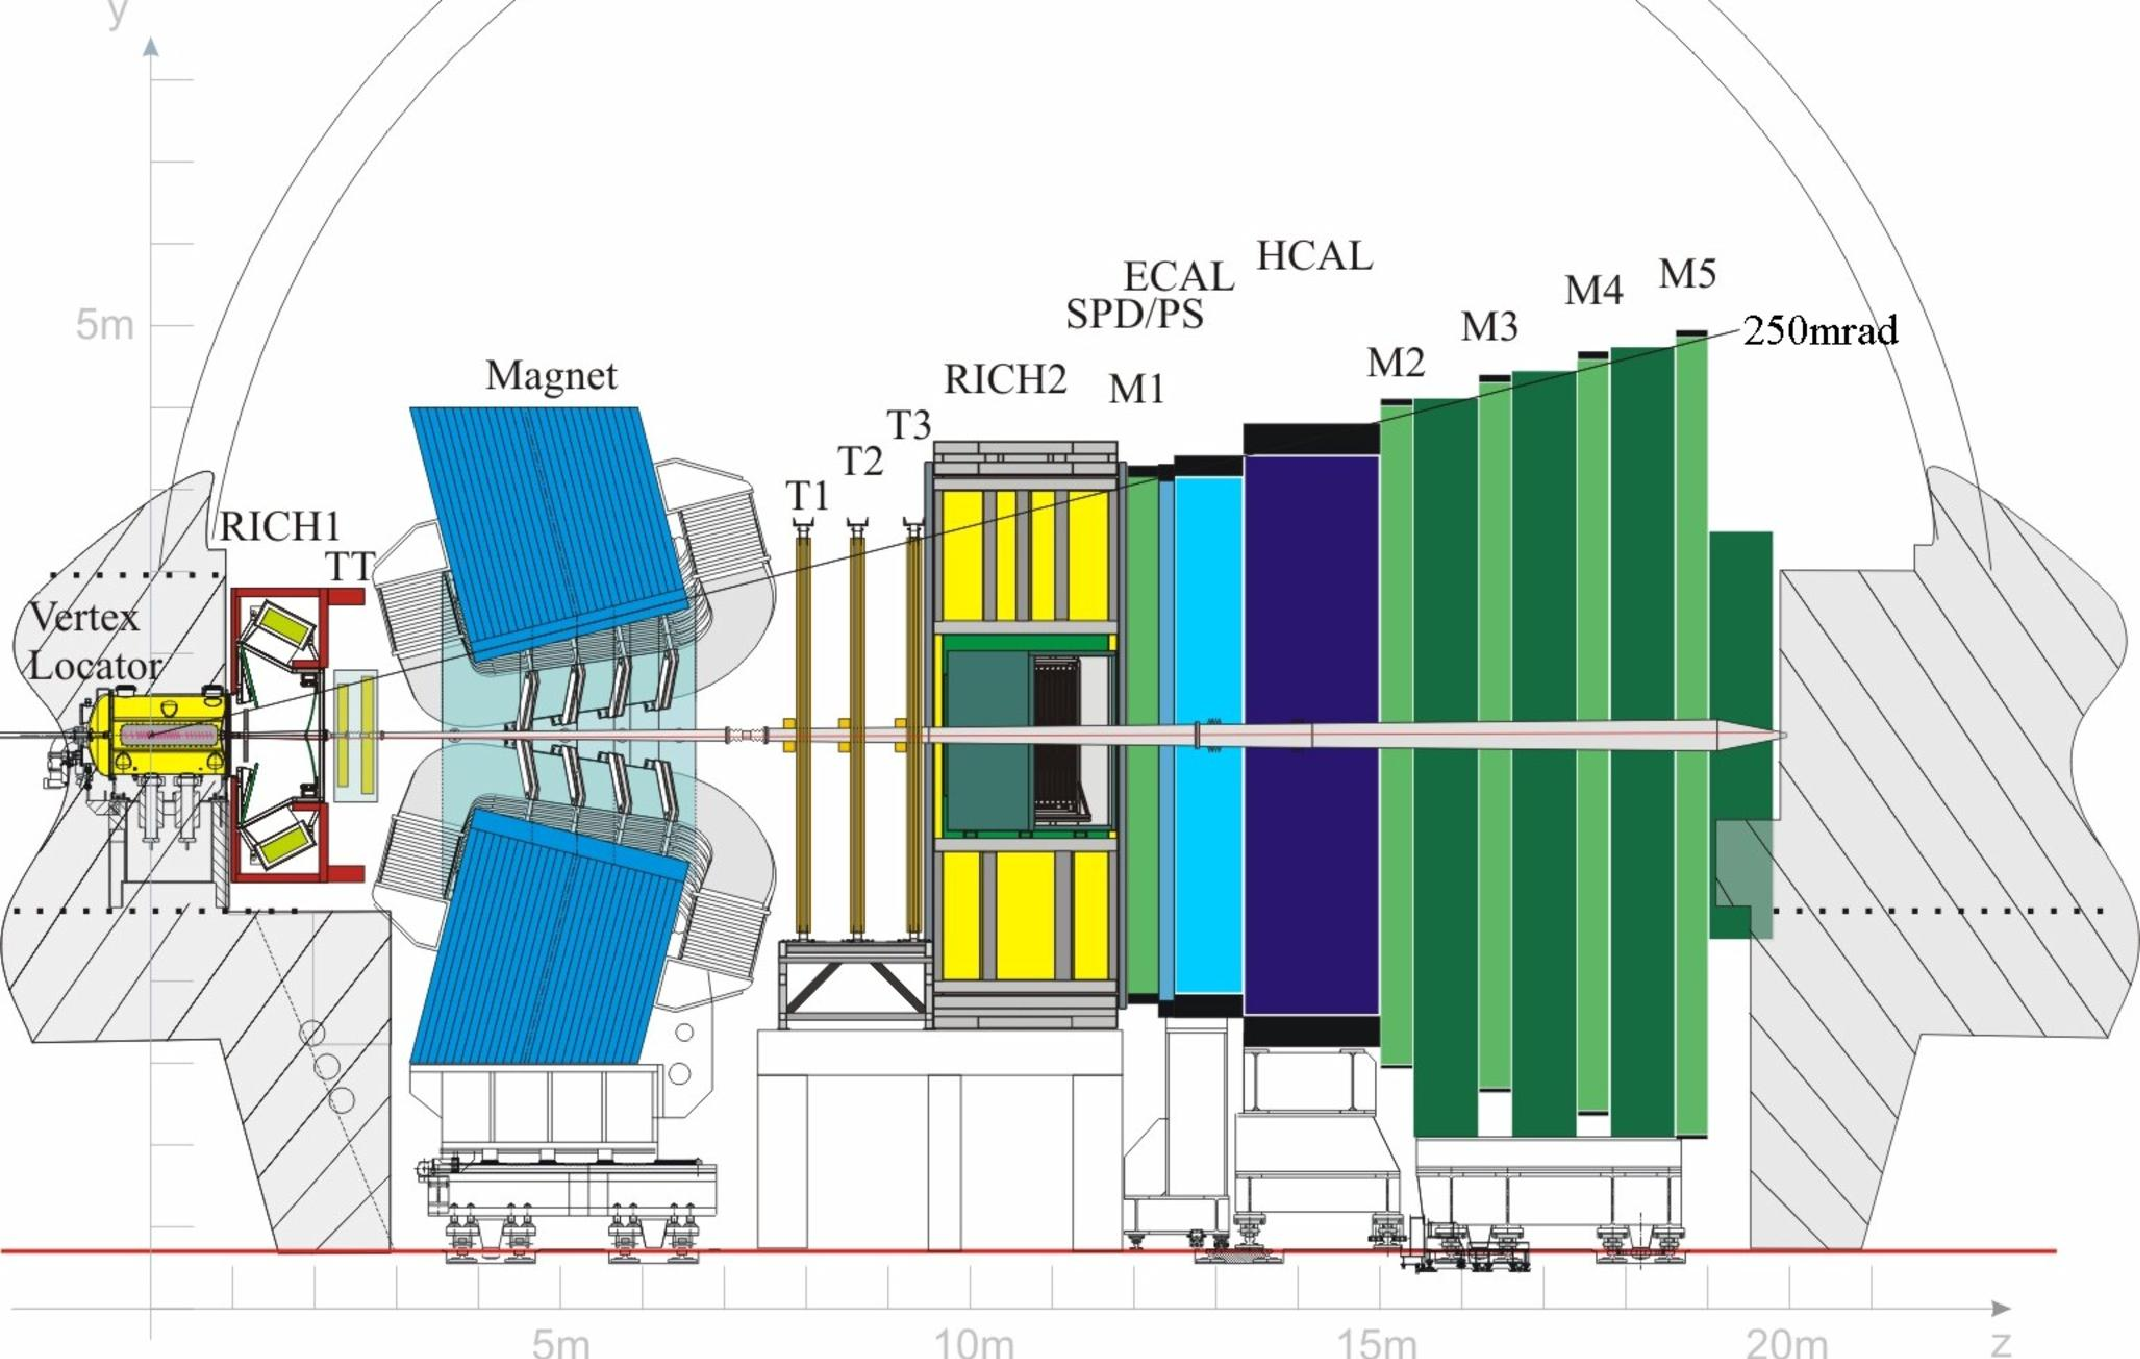
\includegraphics[ width=1.0\textwidth]{LHCb_layout.png}
  \caption{Simulated angular distribution for b-quark production at the LHC, angles are relative the the beam pipe with $\theta =0$ in the forward direction and$\theta = \pi$  in the backward direction \cite{Amato:1998xt}.}
  \label{fig:LHCb_detector}
\end{figure}


\subsection{Tracking}


\subsubsection{VELO}



\begin{figure}[tb] 
  \centering    
  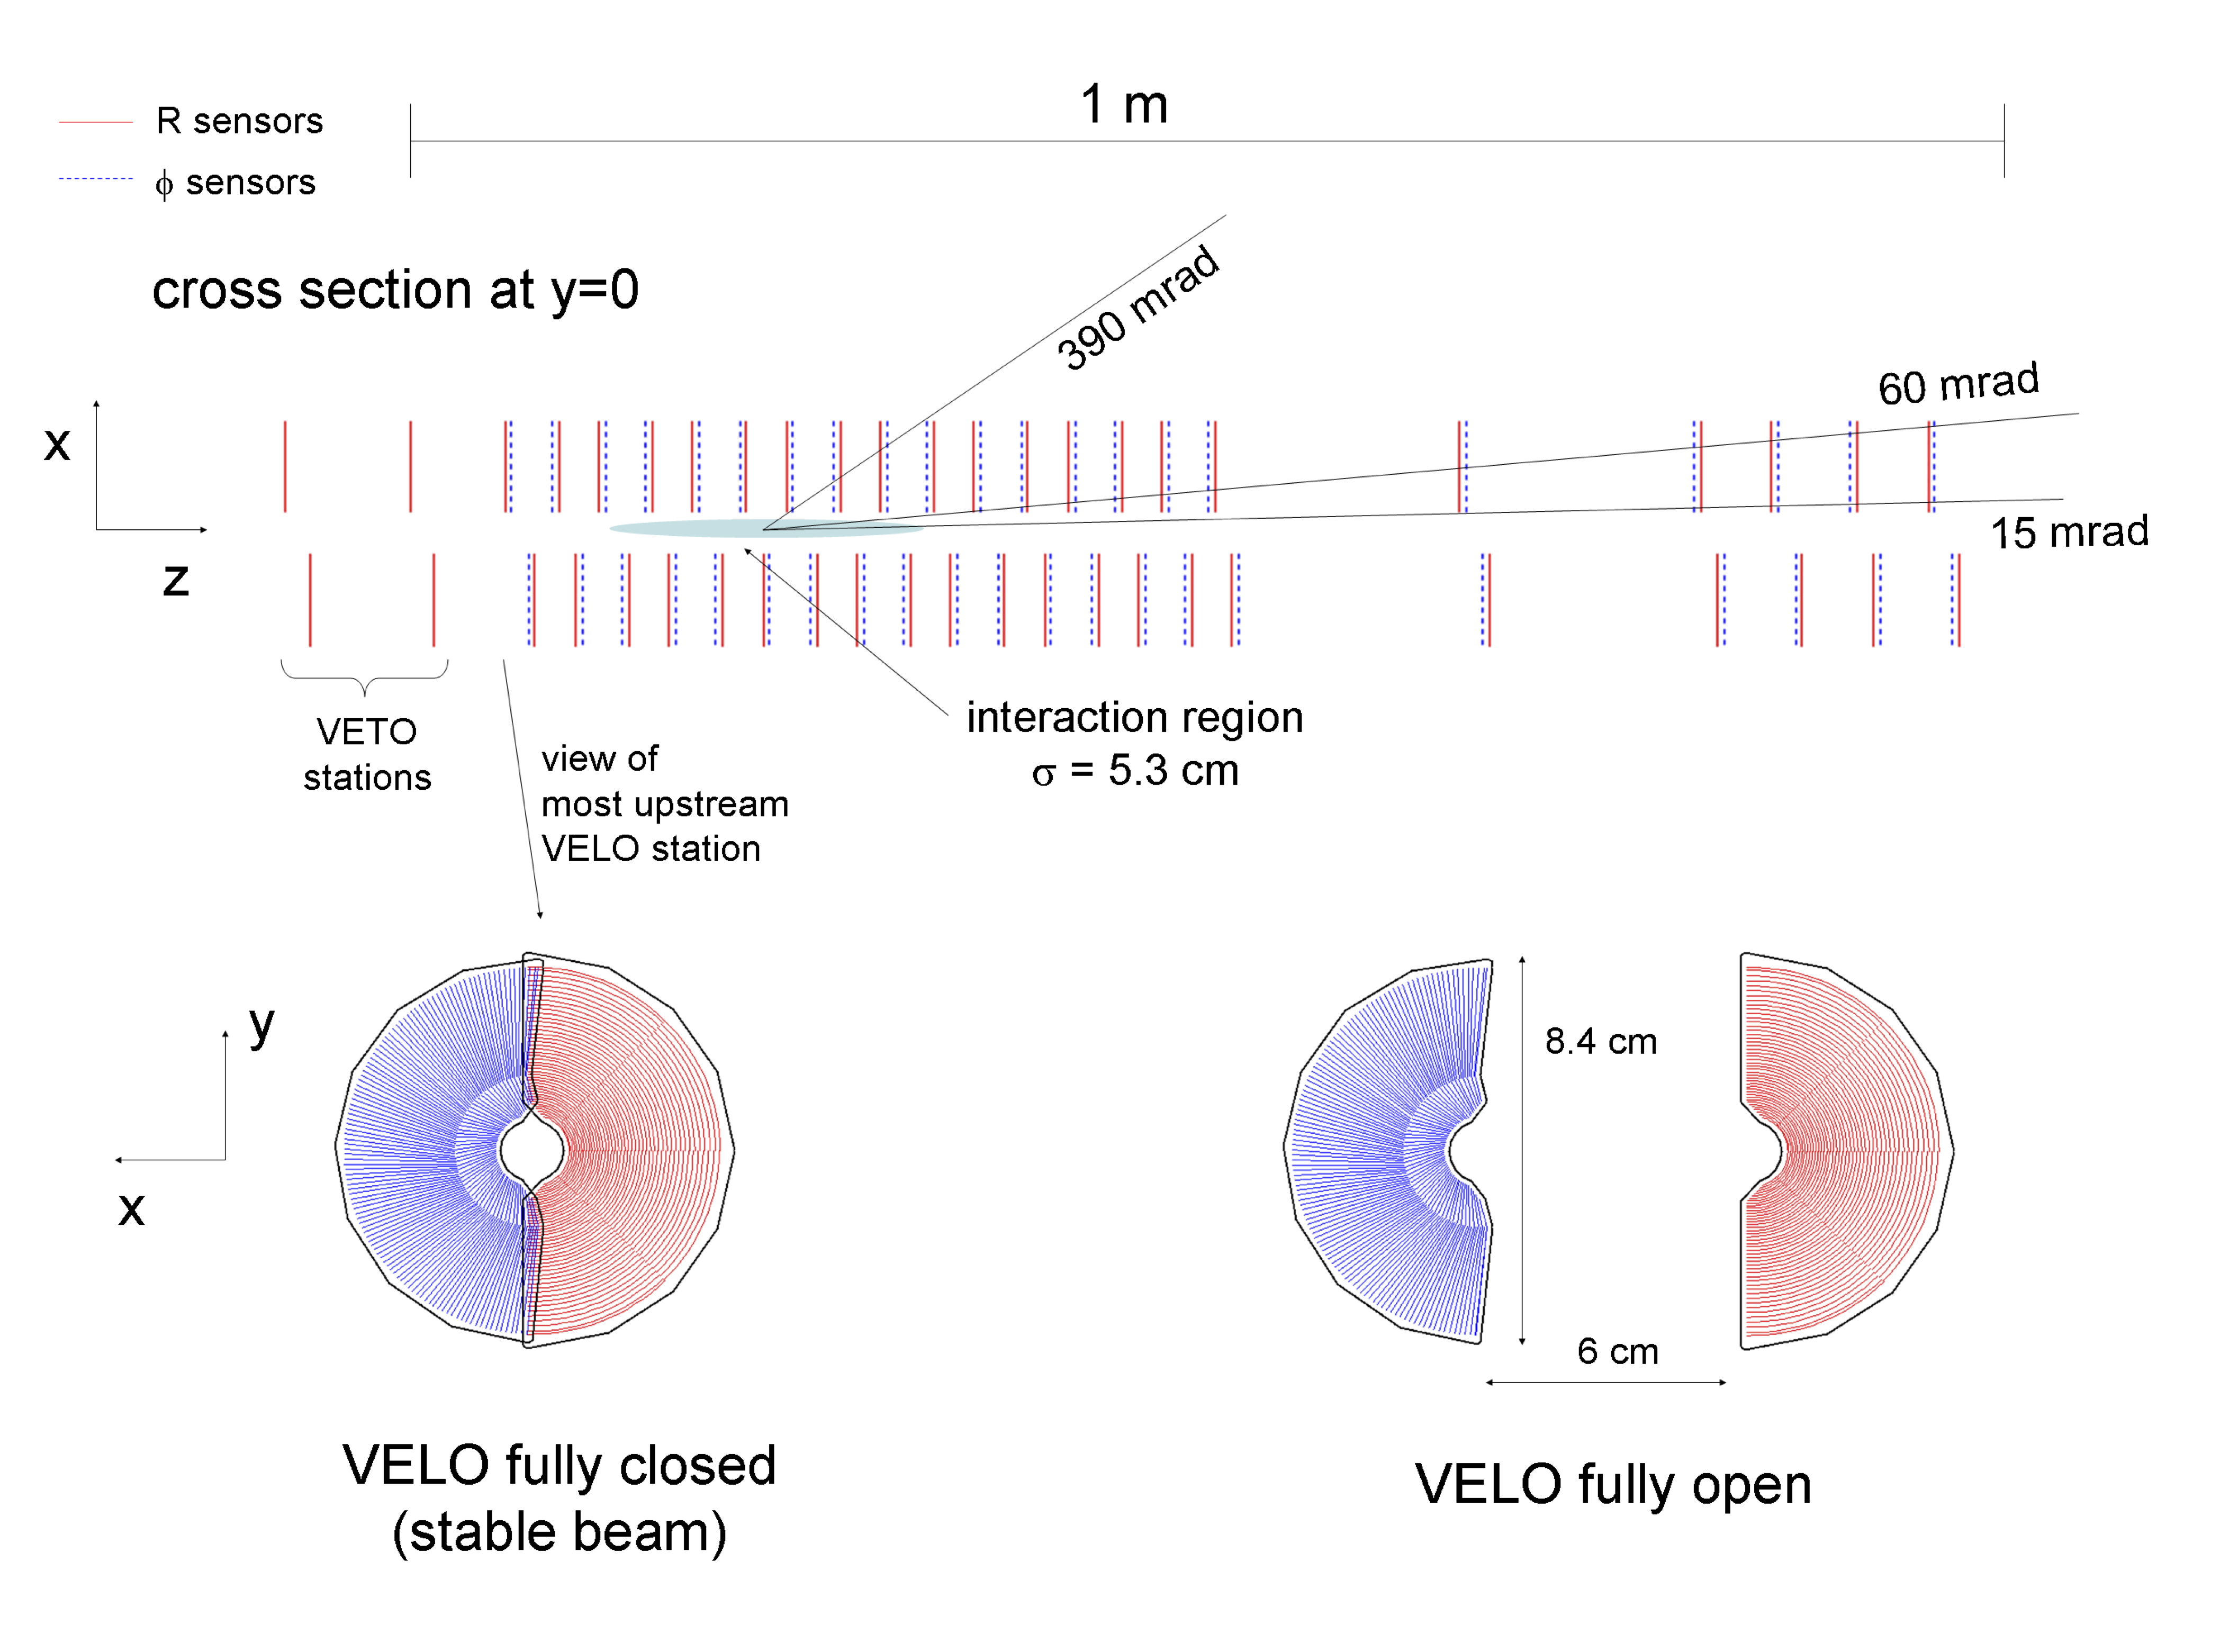
\includegraphics[ width=1.0\textwidth]{velo.png}
  \caption{The velo \cite{Alves:2008zz}.}
  \label{fig:velo}
\end{figure}

\begin{figure}[tb] 
  \centering    
  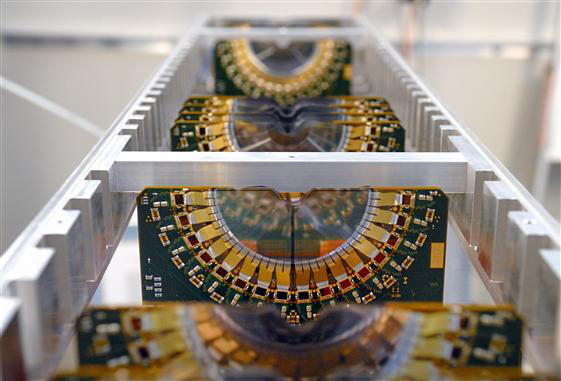
\includegraphics[ width=1.0\textwidth]{Velo_photo.jpg}
  \caption{The velo Soure: LHCb.}
  \label{fig:velo_photo}
\end{figure}

\begin{figure}[tb] 
  \centering    
  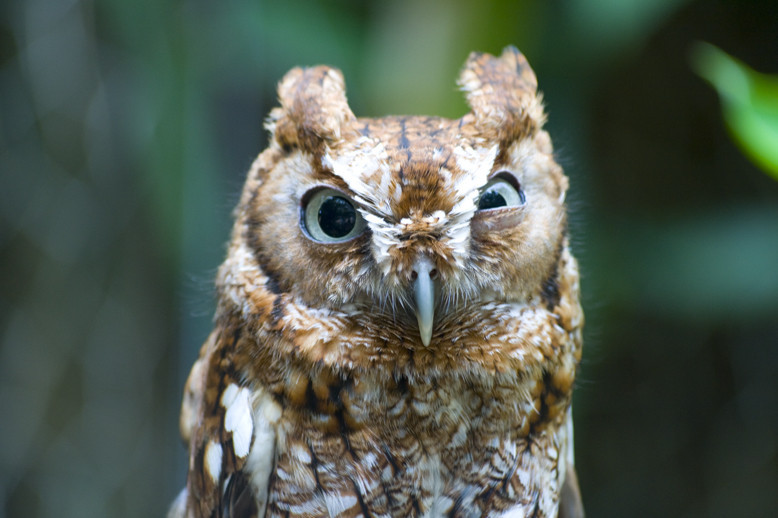
\includegraphics[ width=1.0\textwidth]{placeholder.jpeg}
  \caption{The velo sensor \cite{Alves:2008zz}.}
  \label{fig:velo_sensor}
\end{figure}

\subsubsection{Magnet}

\subsubsection{Tracking Stations} %Or split us the TT and T1-3.

\subsubsection{Track resconstruction and preformance}


\subsection{Particle Identification}
\subsubsection{RICH}
\subsubsection{Calrimeters}
\subsubsection{Muon Stations}
\subsubsection{Combined PID information and performance}

\subsection{Trigger and event filtering}

\subsection{MC and Software}

\subsection{LHCb data collected so far}

\begin{figure}[tb] 
  \centering    
  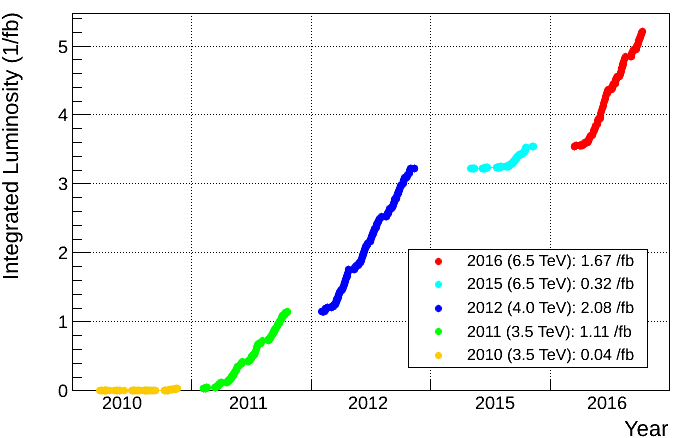
\includegraphics[ width=1.0\textwidth]{IntegratedLumiCumul.png}
  \caption{Source: LHCb.}
  \label{fig:cumulative_lumi}
\end{figure}

\begin{figure}[tb] 
  \centering    
  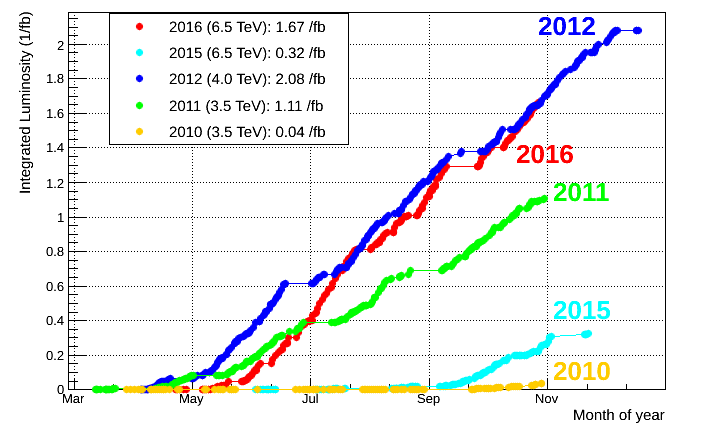
\includegraphics[ width=1.0\textwidth]{IntLumiRun1-2.png}
  \caption{Source: LHCb.}
  \label{fig:yearly_lumi}
\end{figure}
